\documentclass[a4paper]{article}
\usepackage[ngerman]{babel}
\usepackage{amsthm}
\usepackage{amsmath}
\usepackage{amsfonts}
\usepackage{parskip}
\usepackage{graphicx}
\usepackage{color}
\usepackage[hidelinks]{hyperref}
\usepackage{amsthm}
\usepackage{csquotes}

\theoremstyle{definition}
\newtheorem{definition}{Definition}[section]

\hypersetup{linktoc=all,colorlinks=false}

\pagestyle{headings}

\begin{document}
\begin{titlepage}
	\begin{center}

		\Huge
		\textbf{Speedcube-Metrics}

		\vspace{0.5cm}
		\LARGE
		Mobile Applikationen

		\vspace{1.5cm}
		Aaron Schweig, Michael Angermeier, Patrick Mischka,
		Troy Keßler, Jan Grübener

		\vfill

		Studiengang\\
		\textbf{Wirtschaftsinformatik\\ WWI 18 SEAC}

		\vspace{0.8cm}

		Dozent\\
		\textbf{Michael Spengler}

		\vspace{0.8cm}

		\vspace{0.8cm}

		
\includegraphics[width=0.6\textwidth]{img/dhbw.jpg}

		\Large
		DHBW Mannheim\\
		\today

	\end{center}
\end{titlepage}

\tableofcontents
\clearpage

\section{Worum geht es?}
\subsection{Die Idee}
Als Ernő Rubik 1974 den sogennaten Zauberwürfel entwarf wurde das Puzzle zu einem weltweiten Phänomen \cite{ernorubik}.
Millionen von Kindern und Erwachsenen versuchten sich an diesem Rätsel, wobei die Lösung oft als unmöglich
galt. Schließlich kamen erste Lösungsanleitungen wie die Fridrich- oder die Roux-Methode. Damit konnte jeder Würfel
mithilfe weniger Algorithmen gelöst werden. Schnell folgten erste Weltrekorde, der erste offizielle
Weltrekord lag dabei noch bei 22.95 Sekunden, wobei die Zeiten schnell fielen. Heute liegt der Weltrekord für den
3x3 bei unglaublichen 3.47 Sekunden, eine Leistung die Glück und vorallem dediziertes Training erfordert \cite{worldcubeassociation}.

Spätestens mit dem bekannter werden von Speedcubing (dem Lösen eines Zauberwürfels in möglichst kurzer Zeit)
entstanden erste Softwareunterstützungen für Training und Wettkämpfe. Es wurden Algorithmen entwickelt, mit denen
man Zauberwürfel für Wettkämpfe verdrehen kann, sodass diese schwer genug und denoch fair für alle Teilnehmer sind.
Weiterhin wurden erste Apps und Webseiten entwickelt, die diese Wettkämpfe simulieren, sodass man auch von zu
Hause aus seine Fähigkeiten unter Beweis stellen kann. Nach und nach wurden auch weitere Features hinzugefügt,
mit denen man sich eher auf's reine Training konzentrieren konnte.

Wir haben jedoch beobachtet, dass besonders Webbasierte Seiten keine gute User Experience bieten. Das liegt
unter anderem an dem recht altmodischen Design, als auch an fehlenden oder schlecht umgesetzten Features.
Da sich in unserer Gruppe Speedcuber befinden, welche solche Seiten regelmäßig nutzen hatten wir die Idee im
Rahmen dieser Vorlesung eine Webapp zu entwickeln, welche (unserer Meinung nach) eine bessere Alternative zu bestehenden
Angeboten darstellt. Dabei wollen wir auf bestehenden und funktionierenden Methoden aufbauen und mit entsprechenden
modernen Features und Designentscheidungen die User Experience und den Spaß am Speedcubing erhöhen.
\newpage
\section{How to Use?}
\subsection*{Anmeldung und Registrierung}
Beim Starten der App wird der Nutzer zuerst gebeten, sich mit einzuloggen oder zu registrieren.
\vspace{0.25cm}
\begin{center}
	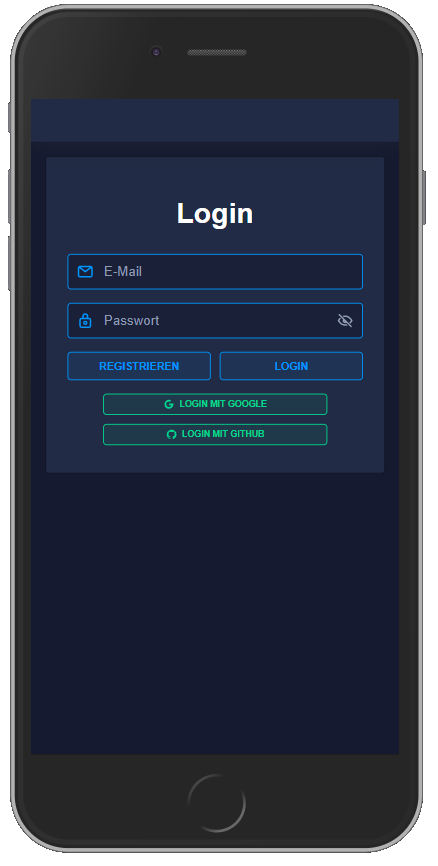
\includegraphics[width= 6cm, keepaspectratio]{img/login}
\end{center}
\vspace{0.25cm}
Er besitzt dabei die Möglichkeit einen Account mittels E-Mail Adresse und eigens gewähltem Passwort zu erstellen oder auf die Autorisierungsdienste von Google oder GitHub zuzugreifen und sich mit seinen bereits vorhandenen Accounts anzumelden. Das bei der Registrierung gewählte verfahren, muss zukünftig auch für jede Anmeldung verwendet werden.
\newpage
\subsection*{Übersicht}
Nach dem erfolgreichen einloggen kann der sieht der Nutzer eine Auswertung seiner letzten Ergebnisse. Hier wird nach Trainings und Wettkämpfen unterschieden und die Ergebnisse des vergangenen Monats graphisch aufgezeigt. So lassen sich Erfolge und Tendenzen schnellstmöglich erkennen.
\vspace{0.25cm}
\begin{center}
	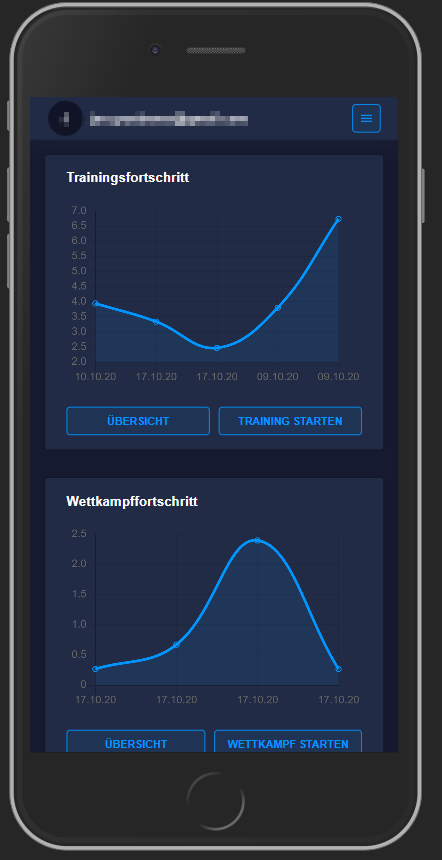
\includegraphics[width= 6cm, keepaspectratio]{img/overview}
\end{center}
\vspace{0.25cm}
Um schnellstmöglich mit dem Spiel beginnen zu können, kann gibt es direkt unter der graphischen Auswertung Buttons um ein Training oder Wettkampf zu starten. Daten interessierte können die Möglichkeit nutzen, sich mit der Hilfe des Übersicht Buttons genauer in ihre erreichten Resultate einzulesen und so sich weiter zu verbessern.
\begin{center}
	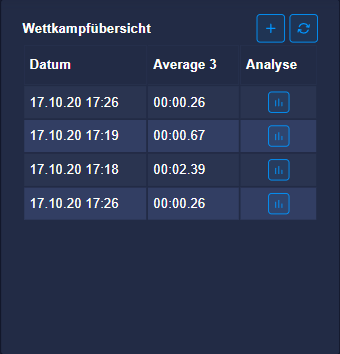
\includegraphics[width= 6cm, keepaspectratio]{img/competitionoverview}
\end{center}
Dafür wird ihnen extra ein eine Tabelle mit den vergangenen Resultaten angezeigt. Für abgeschlossene Trainings wird die jeweilige Lösungszeit des Scrumbels angezeigt. Für absolvierte Wettkämpfe wird hier der Average 3 angezeigt. Über die Spalte Analyse können die Ergebnisse der einzelnen Runden eines Wettkampfes sowieso weitere Daten wie Average 5, Best, Worst, etc. angezeigt werden.
\begin{center}
	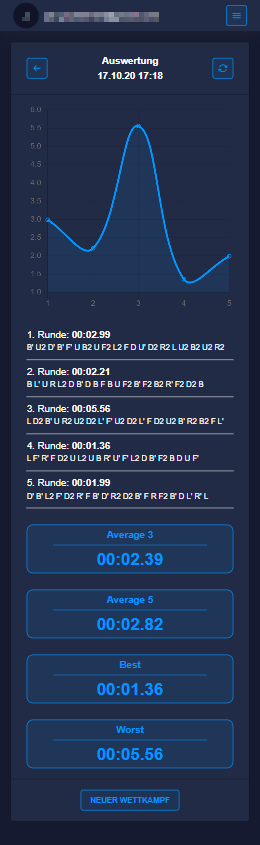
\includegraphics[width= 4cm, height=11cm]{img/competitiondetails}
\end{center}
\newpage
\subsection*{Navigation}
Die Navigation innerhalb der App kann entweder durch die in den einzelnen Abschnitten eingepflegten Buttons erfolgen, die mit einer einfachen Beschreibung zu den logischen nächsten Schritten führen oder über die im Menü eingebundene Navigationsleiste.
\vspace{0.25cm}
\begin{center}
	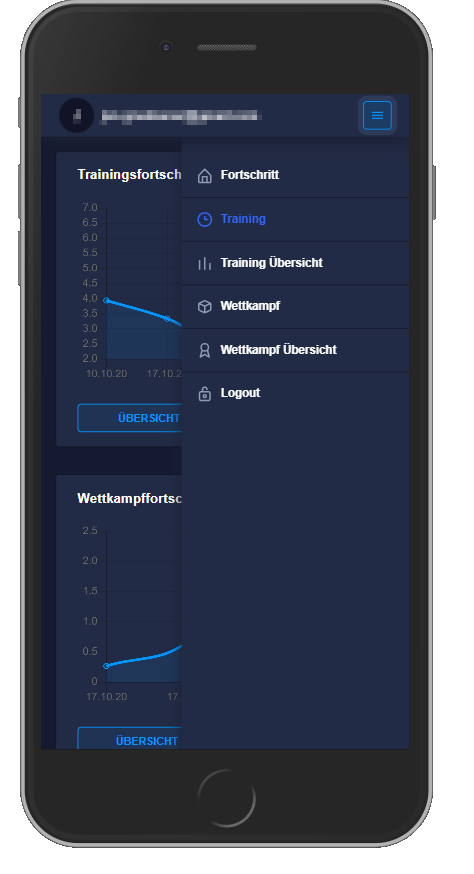
\includegraphics[width= 5cm, keepaspectratio]{img/nav}
\end{center}
\vspace{0.25cm}
Die Navigationsleiste ermöglicht jederzeit das schnelle wechseln zu den Übersichten der letzten Trainings und Wettkämpfe sowie das Starten dieser. Hier findet der Nutzer auch die Möglichkeit vor sich auszuloggen, bevor er die App beendet.
\subsection*{Training}
Ein Training beginnt immer damit, dass die App einen automatisch generierten Scrumpel vorschlägt, welcher im Anschluss der Nutzer auf seinem Rubik´s Cube übernimmt. Dies kann er entweder über den als Text angezeigten Scrumbel oder mithilfe des 3 Dimensional dargestellten Cubes. Zur einfacheren Handhabung und Kontrolle ist dieser durch halten und Bewegungen im Raum dreh und bewegbar. Unpassende Scrumbels können mit dem "Neuer Scrumble" Button einfach übersprungen werden.
\vspace{0.25cm}
\begin{center}
	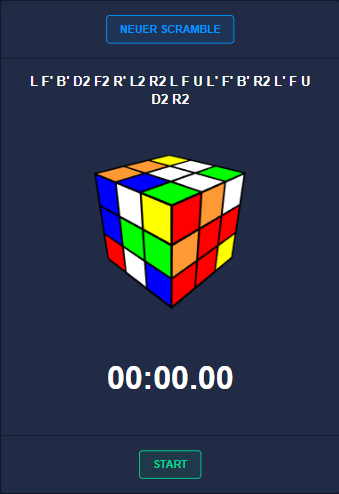
\includegraphics[width= 5cm, keepaspectratio]{img/training}
\end{center}
Der Start Button startet automatisch den eingeblendeten Timer. Wird man bei der Lösung des Scrumbels gestört oder möchte aus anderen Gründen einen neuen Versuch starten, so kann der aktuelle Durchgang durch den Abbrechen Button unterbrochen und der Scrumbel erneut gelöst werden. Stop speichert das Training und bietet sofort einen neuen Scrumbel für einen neuen Versuch.
\vspace{0.25cm}
\begin{center}
	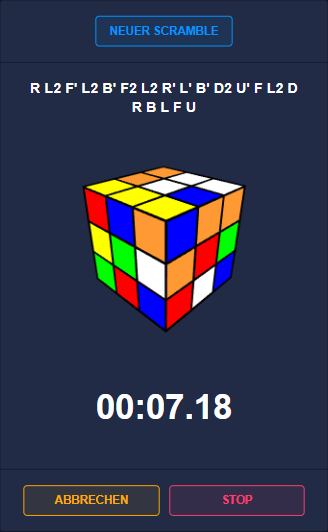
\includegraphics[width= 5cm, keepaspectratio]{img/trainingdone}
\end{center}
\newpage
\subsection*{Wettkampf}
Ein Wettkampf besteht immer aus 5 unterschiedlichen Scrumbels, die schnellstmöglich hintereinander gelöst werden sollen. Das drücken des Stopp Buttons zeigt immer automatisch den nächsten Scrumbel an, der mit dem eigenen Rubiks Cube gelöst werden soll. Hierfür muss der Timer wieder seperat gestartet und gestoppt werden.
\vspace{0.25cm}
\begin{center}
	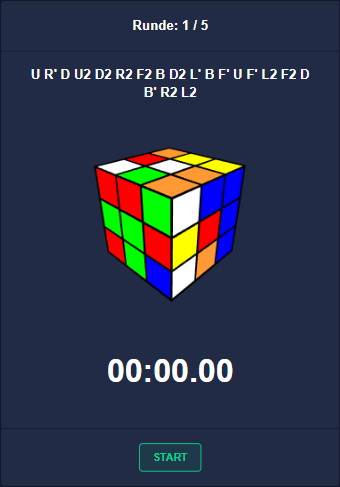
\includegraphics[width= 4.5cm, keepaspectratio]{img/competition}
\end{center}
\vspace{0.25cm}
Nach dem alle 5 Scrumbels gelöst wurden, bekommt der Nutzer die Möglichkeit den Wettkampf zu verwerfen oder ihn zu speichern. Das Verwerfen führt automatisch zu einem neuen Wettkampf mit anderen Scrumbels, das speichern zeigt die Ergebnisse des Wettkampfes an und berechnet wichtige Daten wie Average 4 und Avergage 5 um sich mit alten Wettkämpfen oder Freunden vergleichen zu können.
\begin{center}
	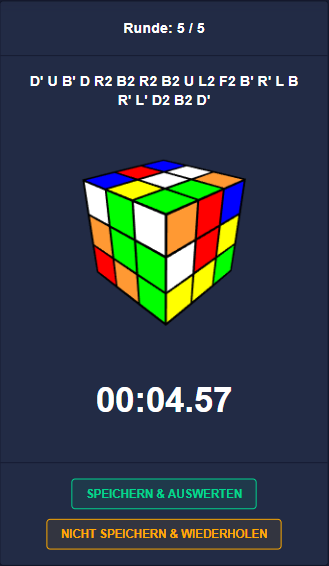
\includegraphics[width= 4.5cm, keepaspectratio]{img/competitiondone}
\end{center}
\section{Technology \& Architecture}
% !TeX root = ./doku.tex

Im folgenden Abschnitt wird kurz die Wahl eines \textbf{BaaS} (Backend as a Service) Anbieters erläuter. Dabei liegt der Fokus vor allem darauf, wieso ein BaaS unter dem gegebenen Anwendungsfall sinnvoll ist.

\subsection{Was ist ein BaaS}
\begin{definition}[Backend as a Service]
    Backend-as-a-Service (BaaS) ist ein Cloud-Service-Modell, bei dem Entwickler alle Hintergrundaspekte einer Web- oder Mobilanwendung auslagern, so dass sie nur das Frontend schreiben und warten müssen. BaaS-Anbieter bieten vorab geschriebene Software für Aktivitäten auf Servern an, z. B. Benutzerauthentifizierung, Datenbankverwaltung, Remote Updates und Push-Benachrichtigungen (für mobile Apps) sowie Cloud-Storage und -Hosting
    \cite{cloudfare}.

    Anhand dieser Definition lässt sich erkennen, dass ein BaaS darauf abzielt, Entwicklungszeiten zu verkürzen und klassische Aufgaben bei der Erstellung einer Webapp zu standardisieren. Zu dem typischen Elementen, die durch BaaS-Anbieter übernommen werden gehören:
    \begin{itemize}
        \item Datenbankverwaltung
        \item Cloud-Speicher
        \item Authentifizierung
        \item Push-Notifications
        \item Hosting
    \end{itemize}

    Es ist zu erkennen, dass so die Entwicklung und die initiale Hürde verloren geht, da elementare Bestandteile einer Webapplikation bereites vorhanden sind und nicht für jeden Anwendungsfall erneut entwickelt werden müssen. Mithilfe einer vorhanden Datenbank und einer sicheren, verwalteten Nutzerauthentifizierung sind bereits Grundsteine gelegt, damit eine Webapp erfolgreich aufgebaut werden kann. Das Modell eines BaaS ist noch nicht sehr alt und wurde innerhalb der letzten Jahre immer populäre. Ereignisse, wie die strikte Regulierung der DSGVO stellt die Nutzung dieser Modelle in einem Enterpreiseumfeld vor Herausforderungen. Diese müssen vor einer Entscheidung für einen solchen Dienst abgewogen werden.

    \subsection{Wieso Firebase?}
    Innerhalb dieses Anwendungsfalles lassen sich verschiedene Aspekte finden, welche für die Nutzung eines BaaS und auch Firebase als populären Anbieter eines solchen Service sprechen.
    \begin{enumerate}
        \item \textbf{Speicherung weniger bis garkeiner nutzerspezifischer Daten:}\\
              In diesem Anwendungsfall werden Nutzerdaten nur gespeichert, damit der eigene Fortschritt visualisiert werden kann. Das bedeutet im Kern, dass außer einer eindeutigen Mailadresse keine zusätzlichen Informationen eines Nutzers benötigt werden. Mithilfe von verschiedenen Social-Auth Providern kann auch eine sichere Authentifizierung gewährleistet werden, da diese immer einem aktuellen Web-Standard - OAuth 2.0 - folgen.
        \item \textbf{kaum speziell im Backend auszuführende Logik:}\\
              Dadurch, dass diese Applikation vorerst rein zum visualisieren des persönliches Fortschritts dient, gibt es sehr wenig Logik, die auf einem Server ausgeführt werden müssten. Durch die direkte Verbindung zwischen Frontend und Datenbank mittels Firebase können Lese- und Schreibanforderungen direkt im Frontend gesteuert werden. Die Logik zum generieren eines zufälligen Scrumbles und zum erstellen des 3D-Cubes wird mithilfe einer \enquote{serverless Function} ausgeführt.
    \end{enumerate}
\end{definition}

\section{Testing}
Aufgrund unserer Wahl für Firebase als Backend sind Backendtests hinfällig und lediglich UI-Tests im Frontend werden benötigt. Hierfür wird \href{https://www.cypress.io/}{cypress} als Testing-Framework genutzt.

Im Rahmen der Frontend-Tests wird zuerst getestet, dass dem Nutzer die korrekte Anmeldemaske angezeigt wird, welche die beiden Anmeldefelder mit Email und Passwort, ein Registrierungsbutton, ein Anmeldebutton und je ein Button um sich mit Google oder Github anmelden zu können, enthalten soll. Desweiteren wird hier getestet ob ein erfolgreiches An- und Abmelden möglich ist.

Nach dem erfolgreichen Anmelden wir die Fortschrittsseite angezeigt, welche sowohl den Trainingsfortschritt, als auch den Wettkampffortschritt enthält. Unter jeder Fortschrittsansicht sind zwei Buttons. Mit einem kann die jeweilige Übersicht detaillierter angezeigt werden, mit dem anderen kann ein Wettkampf / Training gestartet werden.

Das korrekte Öffnen und Schließen des seitlichen Menüs wird ebenfalls getestet. Über dieses Menü können alle weiteren Funktionalitäten der Anwendung erreicht werden. Das Öffnen dieser Funktionalitäten ist ebenfalls getestet.

Die spezifischen Inhalte von den unterschiedlichen Funktionalitäten sind ebenfalls getestet.

\section{Backlog}
Das Backlog beinhaltet alle Features, welche es nicht in die Implementierung geschafft haben. Grund dafür ist
unsere Einschätzung bezüglich des Nutzen-Aufwands.

\begin{itemize}
	\item Eine Berechnung des Lösungsalgorithmus anhand von Image Recognition des Zauberwürfels. Dabei soll der
	      User mithilfe seiner Kamera den Würfel einscannen und die Software den entsprechenden Lösungsalgorithmus
	      berechnen. Die Challenge hier ist das Einscannen des Würfels, da das Training eines Models sehr aufwendig ist
	      (alle Testdaten müssten selbst generiert werden) und die Fehlerquote womöglich aufgrund Belichtung und anderer
	      Einflüsse sehr hoch ist.
	\item Die Berechnung der Umdrehungen pro Sekunde anhand der Geräusche die ein Würfel beim drehen von
	      sich gibt. Dabei ist ein wichtiger, aber auch sehr schwer zu messender Indikator für einen Speedcuber die TPS
	      (Turns per Second). Wir hatten die Idee mithilfe von Audio Recognition Software diese Umdrehungen zu messen
	      und für den User entsprechend darzustellen. Damit kann dann auch berechnet werden, wie flüssig der Speedcuber
	      den Zauberwürfel gelöst hat, indem man sich die Spannweite der TPS betrachtet. Mögliche Challenges wäre hier
	      wieder die Audio Recognition, obwohl diese womöglich wesentlich einfach ist als die Image Recognition. Mögliche
	      Fehlerquellen wären hier störende Hintergrundgeräusche oder der individuelle Klang jedes Würfels.
	\item Das Vergleichen der eigenen Leistung mit Freunden und anderen Nutzern der Webapp. Da Konkurrenz wohl die
	      größte Motivation darstellt sich zu verbessern soll der User die Möglichkeit besitzen seine Leistungen
	      mit allen zu teilen. Dies soll mithilfe einer globalen Rangliste möglich sein. Challenges wären hier die
	      Verifikation, da man ohne weiteres die Zeit stoppen kann und diese veröffentlichen kann.
\end{itemize}

\clearpage

\bibliographystyle{plain}
\bibliography{quellen}

\end{document}